\section{Analytical steps}

Once all our engineered features have been generated from channel 1 and 2, for all log files, we can proceed with our analysis.
Our first step is to characterise noise and signal, so we plot a significant section of both, taken from \textit{Test45.log} and \textit{Test48.log}. Each plot consisting of a 12 second sample approximately. we plot the value of channel 1 (Flame A) in blue and (Flame b) in orange. 

We see from Fig. 2. that in our signal data, both channels are tightly coupled, and there could be a number of different markers to show this, correlation and distance being two possible choices. As a result channel 2 almost hides channel 1. The disturbance in the middle section being a barbecue lighter lit while the UUT was logging.

We then see from Fig. 3. that our noise data shows less overlap and greater distance between both channels, as well as antiphase, so these engineered features could be used charaterise noise. Both channels are mostly visible and both colours can be distinguished.

We now have visual markers for signal and noise, based on our computation. we are now equipped to create additional plots, where antiphase and distance can be added. Fig. 4. has the same plot as Fig. 2 with the added antiphase and distance functions, where it is clear that actual fire signal has no antiphase, the overall distance function being consistently at the lower end of the normalised byte scale. Both markers together can provide a good indication of where a noise attenuating scheme such as linear interpolation would be useful, as can be seen in Fig. 5. with distance and antiphase function plots together with noise. A next step in visualisation can be seen in Fig. 6. where the channels 1 and 2 are removed from the plot, and the area under the distance function is highlighted in green. We now, using this scheme, apply linear interpolation to minimise areas under the function, obtaining data to generate plots and lines of best fit, together with correlation coefficients. Nothing again that we are not interested in the value of $ r^2 $, as correlation coefficient is used as a proxy for distance.
The stopping condition for our linear interpolation algorithm being the best threshold \textit{t}, preserving signal while eliminating most of the noise.
Visual analytics motivated the search for a second attenuation algorithm (linear interpolation), as visually is was clear that mearly smoothing a signal would not minimise the distance or antiphase functions.

We created 3 series of 6 sample plots for the original normalised data, Savistzky-Golay filtered data and Linear Interpolation smoothed data, in Fig. 7., Fig. 8. and Fig. 9. respectively, showing best lines of fit, together with correlation coefficients, these should help inform which schemes work best.

Note no channel 1 and channel 2 plots are shown here for the Savistzky-Golay filter or linear interpolation filter, for the sake of keeping a good balance between text and images. It is worth mentioned that the stopping condition for the Savitzky-Golay filter is found based on experimentations with the window length and polynomial order, and are an artifact of previous work \cite{Sikar:INM430}. Note these values where obtained empirically, and not though a specific computational technique.

The last piece of computation and visual methods is the more traditional Table 1., with an asterisk denoting which scheme provided the highest correlation coefficient, minimising the distance between channel 1 and channel 2 and as a consequence, attenuating the noise. 

\begin{figure}[tb]
 \centering % avoid the use of \begin{center}...\end{center} and use \centering instead (more compact)
 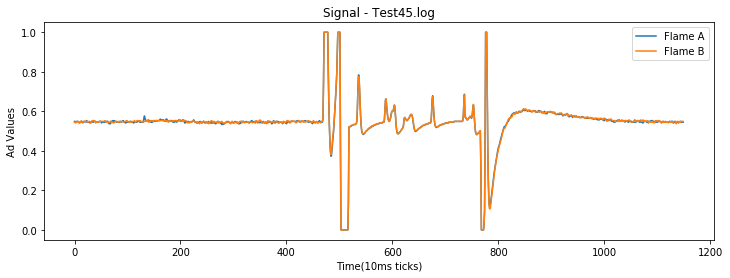
\includegraphics[width=\columnwidth]{pictures/05-signal.png}
 \caption{Characterising noise and signal - Signal data, generated by waving a barbecue lighter in front of UUT}
 \label{fig:sample}
\end{figure}



\begin{figure}[tb]
 \centering % avoid the use of \begin{center}...\end{center} and use \centering instead (more compact)
 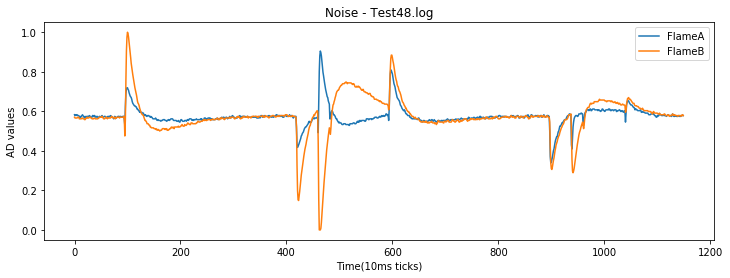
\includegraphics[width=\columnwidth]{pictures/04-noise.png}
 \caption{Characterising noise and signal - Noise data, generated by subjecting UUT to RF interference}
 \label{fig:sample}
\end{figure}

\begin{figure}[tb]
 \centering % avoid the use of \begin{center}...\end{center} and use \centering instead (more compact)
 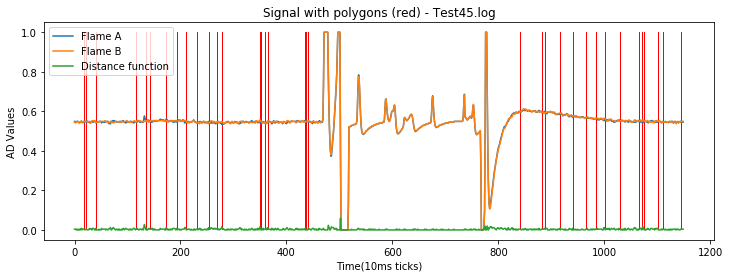
\includegraphics[width=\columnwidth]{pictures/06-signal-antiphase-distance.png}
 \caption{Signal plot with distance and antiphase functions.}
 \label{fig:sample}
\end{figure}

\begin{figure}[tb]
 \centering % avoid the use of \begin{center}...\end{center} and use \centering instead (more compact)
 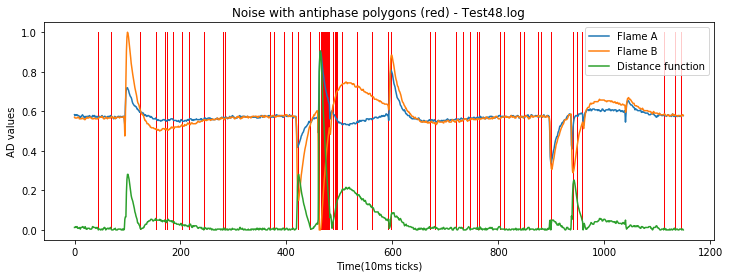
\includegraphics[width=\columnwidth]{pictures/07-noise-antiphase-distance.png}
 \caption{Noise plot with distance and antiphase functions.}
 \label{fig:sample}
\end{figure}

\begin{figure}[tb]
 \centering % avoid the use of \begin{center}...\end{center} and use \centering instead (more compact)
 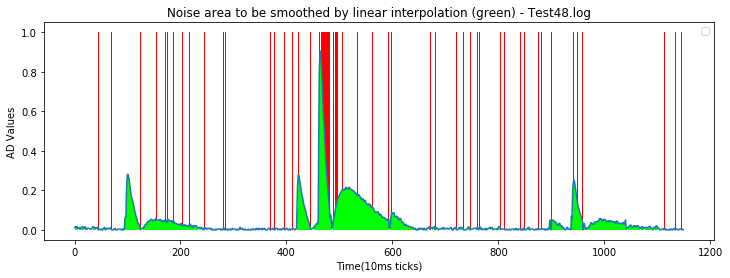
\includegraphics[width=\columnwidth]{pictures/08-noise-linear-interpolation-smoothing.png}
 \caption{Noise plot with area to be smoothed by linear interpolation.}
 \label{fig:sample}
\end{figure}

\begin{figure}[tb]
 \centering % avoid the use of \begin{center}...\end{center} and use \centering instead (more compact)
 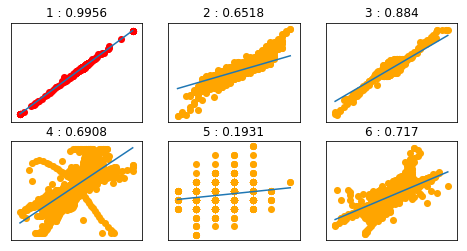
\includegraphics[width=\columnwidth]{pictures/01-raw-linear-regression.png}
 \caption{Linear Regression for 6 sample log files, with lines of best fit and correlation coefficients for normalised data. Top left plot (1) is real fire data, remaining plots contain interference data}
 \label{fig:sample}
\end{figure}

\begin{figure}[tb]
 \centering % avoid the use of \begin{center}...\end{center} and use \centering instead (more compact)
 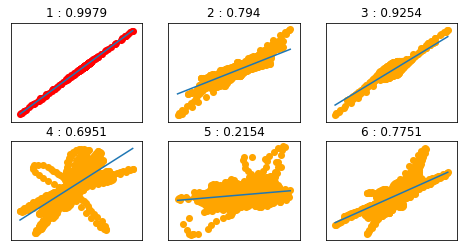
\includegraphics[width=\columnwidth]{pictures/02-sg-linear-regression.png}
 \caption{Linear Regression for 6 sample log files, with lines of best fit and correlation coefficients for Savitzky-Golay filtered data. Top left plot (1) is real fire data, remaining plots contain interference data.}
 \label{fig:sample}
\end{figure}

\begin{figure}[tb]
 \centering % avoid the use of \begin{center}...\end{center} and use \centering instead (more compact)
 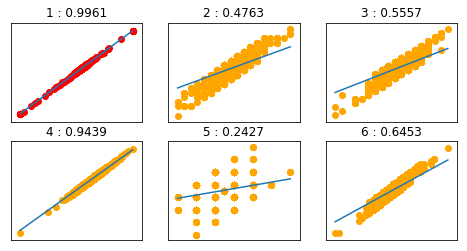
\includegraphics[width=\columnwidth]{pictures/03-li-linear-regression.png}
 \caption{Linear Regression for 6 sample log files, with lines of best fit and correlation coefficients for linear interpolation smoothed data. Top left plot (1) is real fire data, remaining plots contain interference data.}
 \label{fig:sample}
\end{figure}

